\section{Experiments}
\label{sec:experiments}

\subsection{Experimental Setup}
\label{sec:setup}

We study iterative training collapse using Pythia-410M~\citep{biderman2023pythia} as the primary architecture.
Training data is drawn from WikiText-103~\citep{merity2017pointer} following the replace paradigm of~\citet{shumailov2024curse}: each generation fine-tunes on a mixture of $\alpha$ synthetic and $(1{-}\alpha)$ real data, generates 5{,}000 replacement samples, and fully replaces the synthetic pool (hyperparameters in Appendix~\ref{app:training_details}).
We run $T{=}10$ generations across 13 contamination levels ($\alpha \in \{0.00, \ldots, 1.00\}$) with multi-seed replication, yielding ${\sim}1{,}500$ statistical tests after BH-FDR correction~\citep{benjamini1995controlling}.
We track two \emph{canary metrics} (token entropy and ECE) and three \emph{downstream metrics}: distinct-1, distinct-2~\citep{li2016diversity}, and perplexity (distinct-3: Appendix~\ref{app:distinct3}).
PermG uses 5{,}000 permutations on first-differenced series~\citep{shojaie2022granger} with maximum lag~5.


\subsection{Sharp Detection Onset}
\label{sec:regime}

Diversity collapse occurs at every contamination level: distinct-1 declines by $14.1\%$ even at $\alpha{=}0.0$ (fine-tuning drift) and by $40.3{\pm}0.3\%$ at $\alpha{=}0.25$.
Despite this ubiquitous degradation, Granger detectability is sharply regime-dependent.
PermG finds 0/8 canary$\to$downstream pairs FDR-significant from $\alpha{=}0.00$ through $\alpha{=}0.45$, then jumps to 6/8 (Clopper--Pearson 95\% CI $[0.25, 0.92]$) at $\alpha{=}0.50$, uniformly across all 3~fp32 seeds.

\begin{figure}[t]
\centering
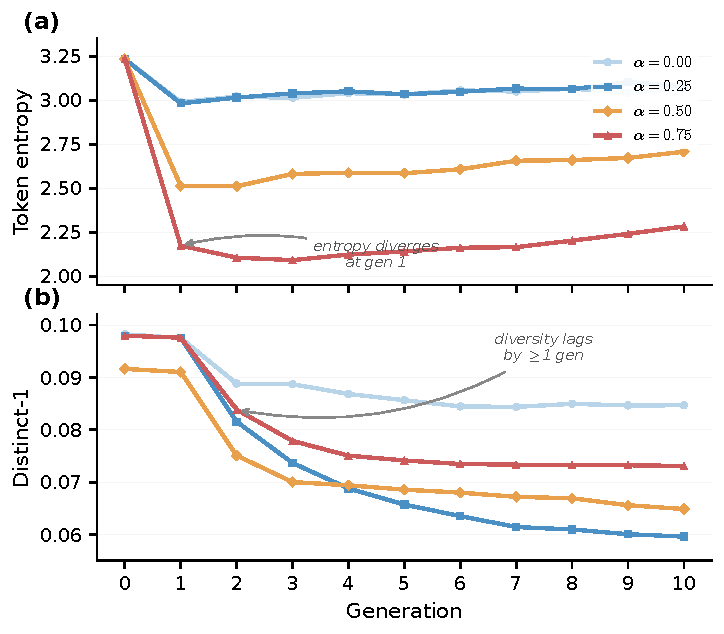
\includegraphics[width=\columnwidth]{figures/metric_trajectory.pdf}
\caption{Metric trajectories at $\alpha{=}1.0$ (Pythia-410M, 4~seeds). Token entropy drops at generation~1; distinct-1 declines from generations~2--3, with a consistent one-generation canary lead (shaded: inter-seed range).}
\label{fig:metric_trajectory}
\end{figure}

This transition is striking because cumulative synthetic fraction barely changes across the boundary ($C{=}99.75\%$ at $\alpha{=}0.45$ vs.\ $99.90\%$ at $\alpha{=}0.50$), yet detection jumps from null to reliable.
Sub-threshold $p$-values at $\alpha{=}0.45$ ($p_{\mathrm{fdr}} = 0.059$--$0.091$) confirm proximity to the boundary.
Sigmoid regression yields $\alpha_c = 0.483 \pm 0.006$ ($R^2 = 0.969$; Figure~\ref{fig:dose_response}); cross-seed consistency (3/3 seeds: $0/8{\to}6/8$) and specification-invariance across 1{,}160 configurations (Appendix~\ref{app:spec_curve}) argue for a genuine transition (Fisher exact: $p = 3.45 \times 10^{-11}$).

First-differencing scopes this canary claim precisely: canary$\to$diversity pairs retain unanimous FDR significance ($24/24 \to 24/24$ across 4~seeds at $\alpha{=}1.0$), while canary$\to$perplexity collapses entirely ($F \approx 0$, $p = 0.99$)~\citep{granger1974spurious}.
At $\alpha{=}1.0$, all 24 canary$\to$diversity pairs reach FDR significance in the forward direction with 0/24 reverse; entropy onset at generation~1 precedes distinct-$n$ at generation~2 in 16/18 WikiText conditions (Appendix~\ref{app:moment_cascade}).
Yet despite this clear signal above onset, a substantial blind zone exists below it: at $\alpha{=}0.10$, distinct-1 has already dropped by $39.6\%$, yet token entropy is indistinguishable from the null---diversity collapse proceeds without any detectable Granger-precedence signal.

\begin{figure}[t]
\centering
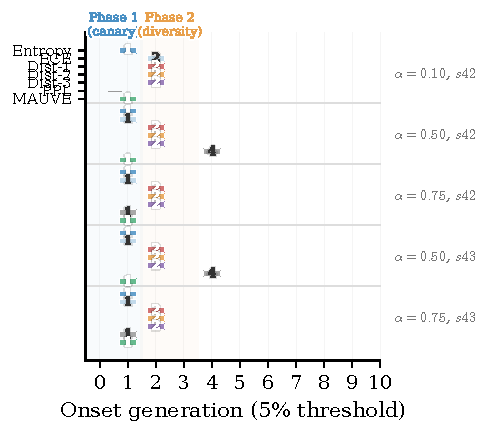
\includegraphics[width=\columnwidth]{figures/fig_cascade_onset.pdf}
\caption{Cascade onset timeline (Pythia-410M, WikiText, fp32). Entropy and ECE reach onset at generation~1; distinct-$n$ follows at generation~2. The ordering $t_H \leq t_D$ holds across all conditions.}
\label{fig:cascade_onset}
\end{figure}

\begin{table}[t]
\centering
\caption{Detection outcomes across contamination levels (Pythia-410M, seed~42, $T{=}10$, fp32). PermG: forward FDR-significant pairs; $K{\geq}3$: consensus pairs (of 8 canary$\to$downstream pairs).}
\label{tab:summary_detection}
\begin{tabular}{@{}lccc@{}}
\toprule
$\alpha$ & PermG & $K{\geq}3$ & Regime \\
\midrule
0.00 & 0/8 & 0/8 & null \\
0.25 & 0/8 & 0/8 & blind \\
0.45 & 0/8 & 0/8 & blind \\
0.50 & 6/8 & 6/8 & onset \\
0.60 & 0/8 & 0/8 & anomaly \\
0.75 & 6/8 & 6/8 & detection \\
1.00 & 6/8 & 6/8 & detection \\
\bottomrule
\end{tabular}
\end{table}

\begin{figure}[t]
\centering
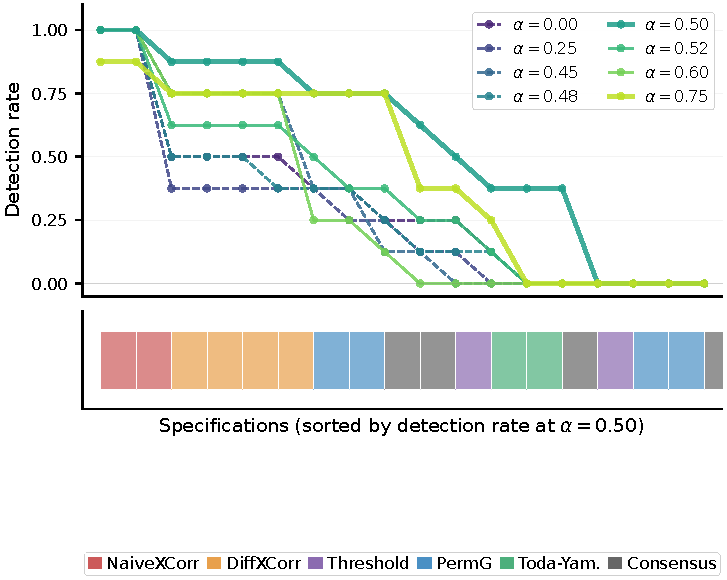
\includegraphics[width=\columnwidth]{figures/fig_spec_curve.pdf}
\caption{Specification curve (1{,}160 configurations). The blind$\to$onset jump at $\alpha_c{\approx}0.50$ is robust across methods, pairs, and seeds.}
\label{fig:spec_curve}
\end{figure}


\subsection{Dose-Response and Detection Regimes}
\label{sec:dose_response}

The PermG dose-response profile (Figure~\ref{fig:dose_response}; Appendix~\ref{app:dose_response}) reveals three confirmed regimes---\emph{blind} ($\alpha \leq 0.45$, 0/8), \emph{onset} ($\alpha \approx 0.50$, 6/8), and \emph{detection} ($\alpha{\geq}0.75$, 6/8)---plus a non-monotonic anomaly at $\alpha \approx 0.60$ (0/8).
The blind zone exhibits zero detection across all seeds and methods below $\alpha{=}0.45$, despite substantial diversity loss---a regime where collapse proceeds silently.
Onset is remarkably steep: the sigmoid Hill coefficient $k{=}15.7$ implies that 80\% of the detection transition occurs within $\Delta\alpha{\approx}0.05$, approximately $3$--$4{\times}$ steeper than smooth-signal predictions (Appendix~\ref{app:power_sim}).
Above onset, the detection zone shows cross-seed consistency: all 3~fp32 seeds independently reach 6/8 at $\alpha{=}0.50$ and $\alpha{\geq}0.75$.

At $\alpha{\approx}0.60$, all direction-checked methods fail (PermG 0/8, threshold onset 0/8, Toda--Yamamoto 1/8), while bidirectional DiffXCorr maintains detection (6/8).
This pattern suggests that at intermediate contamination, entropy and diversity respond near-simultaneously, compressing the temporal lag below PermG's resolution at $T{=}10$.
The anomaly dissolves by $T{=}25$ ($5/8$), consistent with $\sqrt{T}$ power scaling restoring directional separation as additional observations accumulate (Appendix~\ref{app:t20_comparison}).

\subsection{Detection Boundary Left-Shift}
\label{sec:t20}

Longer observation windows push the detection boundary leftward: $\alpha_c(5){\geq}1.0$, $\alpha_c(10){=}0.487$, consistent with power-law scaling $\alpha_c(T) \propto T^{-\gamma}$ (\S\ref{sec:theory}).
Profile likelihood yields $\gamma \in [0.64, 2.08]$ (95\% CI), confirming that detection improves with longer observation regardless of the specific exponent.
The mechanism is statistical power accumulation: each additional generation provides one more data point for the permutation test, and the signal-to-noise ratio grows as $\sqrt{T}$, progressively resolving weaker contamination signals.
The $\alpha{=}0.45$ column validates this prediction directly: undetectable at $T{\leq}10$ (0/8), it crosses into reliable detection at $T{=}15$ (6/8, dual-seed) and remains stable at $T{=}20$ (5/8) and $T{=}25$ (6/8), precisely traversing the blind$\to$detection boundary as the theory predicts.

\begin{figure}[t]
\centering
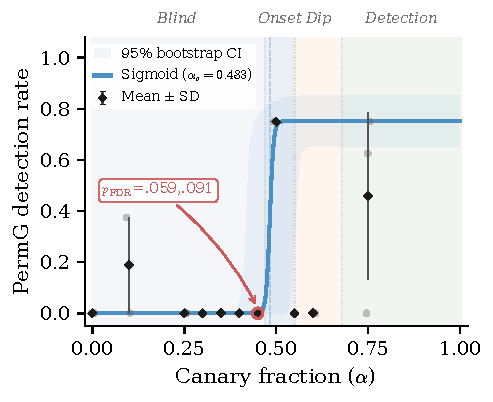
\includegraphics[width=\columnwidth]{figures/fig_dose_response.pdf}
\caption{Dose-response: PermG detection rate with sigmoid fit ($\alpha_c{=}0.483$; shaded 95\% CI). Regime bands mark blind, onset, sync-dip, and detection zones.}
\label{fig:dose_response}
\end{figure}


\subsection{Cross-Architecture Evaluation at $\alpha{=}1.0$}
\label{sec:generalization}

The phase diagram (Figure~\ref{fig:phase_diagram}) characterizes detectability on Pythia-410M + WikiText-103; this section tests whether the detection signal generalizes across architectures at the most favorable contamination level ($\alpha{=}1.0$).
We evaluate PermG across 15 model-seed combinations spanning five families (345M--6.9B) and two domains (Table~\ref{tab:generalization}; Appendix~\ref{app:cross_arch_table}).
Forward detection reaches ${\geq}6/8$ in 11/15 conditions (Figure~\ref{fig:cross_arch_heatmap}).

At larger scale, Pythia-1.4B qualitatively reproduces the 410M phase-diagram structure---detection boundary at $\alpha_c{\approx}0.50$, cross-$T$ improvement at 3/4 $\alpha$ values ($\alpha{=}0.45$: $0/6{\to}5/6$ from $T{=}10$ to $T{=}15$)---though the 410M sync-dip at $\alpha{=}0.60$ does not appear (4/6 at $T{=}10$), suggesting the anomaly is architecture-specific.
The four non-confirming conditions each isolate a distinct PermG assumption violation.
\emph{Precision sensitivity}: GPT-2 bf16 yields 0/8 vs.\ fp32 6/8, traced to bf16 quantization noise masking the entropy signal.
\emph{Bidirectional confounding}: GPT-2 s43 detects 6/8 in both forward and reverse directions, preventing directional assignment.
\emph{Seed dependence}: Pythia-1.4B shows s42 2/8 vs.\ s43 6/8; seed-specific bidirectional confounding also appears at 1.4B (s43 reverse detection 6/8 at $\alpha{=}0.60$), analogous to the GPT-2 case, preventing directional assignment for that seed.
\emph{Entropy decoupling}: SmolLM3-3B reaches only 3/8, with ECE-only detection (entropy 0/4), violating the entropy-leads assumption of Design Principle~\ref{thm:entropy_leads}.
Standalone PermG claims therefore require architecture-specific null calibration; GPT-2 null FPR reaches 50\% (Appendix~\ref{app:fpr_independence}), driven by ${\sim}4{\times}$ stronger null drift than Pythia.

\begin{figure}[t]
\centering
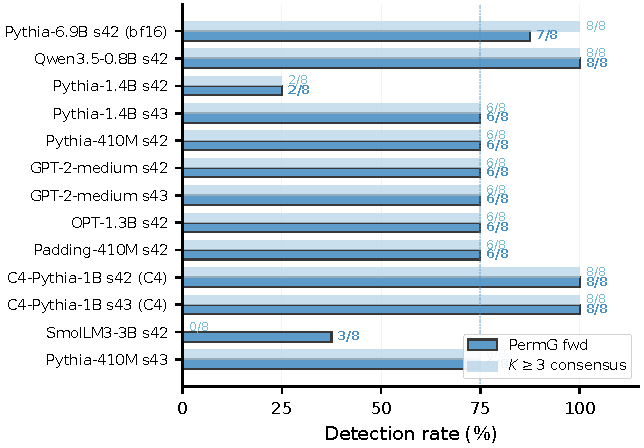
\includegraphics[width=\columnwidth]{figures/fig_cross_arch_heatmap.pdf}
\caption{Cross-architecture validation ($\alpha{=}1.0$): PermG forward detection (${\geq}6/8$) in 11/15 model-seed conditions spanning five families (345M--6.9B); faded bars: non-confirming conditions.}
\label{fig:cross_arch_heatmap}
\end{figure}


\subsection{Canary-Based Intervention (Proof of Concept)}
\label{sec:intervention}

As a proof-of-concept under favorable conditions ($\alpha{=}1.0$), we implement predictive cessation: training switches to pure real data when token entropy drops beyond a 15\% threshold from generation~0 (robust band $[10\%, 22\%]$; Appendix~\ref{app:intervention_sensitivity}).
The predictive trigger fires at generation~1, one full generation before a reactive baseline that monitors distinct-1 directly (which manifests only at generation~2 due to the cascade lag).
Predictive cessation caps peak perplexity at $56.99$ vs.\ $157.09$ reactive, a 64\% reduction (Figure~\ref{fig:intervention}); the result replicates on Pythia-1.4B with comparable effect size (Appendix~\ref{app:extended_discussion}).

\begin{figure}[t]
\centering
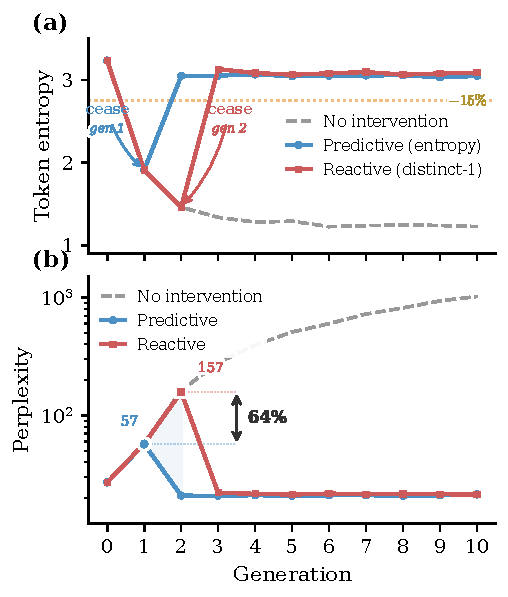
\includegraphics[width=\columnwidth]{figures/fig_intervention.pdf}
\caption{Canary-triggered intervention (Pythia-410M, $\alpha{=}1.0$). Predictive cessation on entropy (generation~1) reduces peak perplexity by 64\% versus reactive triggering on distinct-1 (generation~2).}
\label{fig:intervention}
\end{figure}

\begin{table}[t]
\centering
\caption{Consensus threshold operating characteristics ($K \in \{2,3,4,5\}$). FPR: null-control rate (10~seeds, 60~pairs; $K{\geq}2$ uses 9-seed estimate). TPR: detection rate at selected $\alpha$ levels (Pythia-410M, $T{=}10$, fp32). $K{=}3$ balances FPR control against detection power (75\% at $\alpha{=}1.0$); $K{=}4$ eliminates false positives but reduces TPR to ${\leq}25\%$.}
\label{tab:mmct_k_operating}
\begin{tabular}{@{}lcccc@{}}
\toprule
& $K{\geq}2$ & $K{\geq}3$ & $K{\geq}4$ & $K{=}5$ \\
\midrule
FPR ($\alpha{=}0.0$) & 38.9\% & 10.0\% & 0\% & 0\% \\
TPR ($\alpha{=}0.50$) & 85.4\% & 66.7\% & 25.0\% & 4.2\% \\
TPR ($\alpha{=}0.75$) & 72.9\% & 37.5\% & 0\% & 0\% \\
TPR ($\alpha{=}1.0$) & 75.0\% & 75.0\% & 25.0\% & 0\% \\
\bottomrule
\end{tabular}
\end{table}
